\documentclass[12pt,a4paper]{article}
\usepackage[czech]{babel}
\usepackage[utf8]{inputenc}
\usepackage[T1]{fontenc}
\usepackage{lmodern}
\usepackage{graphicx}
\usepackage{multicol}
\usepackage{titling}
\textwidth 16cm \textheight 24.6cm
\topmargin -1.3cm
\oddsidemargin 0cm
\begin{document}
\pagestyle{empty}
\title{Úlohy na procvičení funkcí}
\date{\vspace{-10ex}}
\setlength{\droptitle}{-6em}
\maketitle

\setlength\parindent{0pt}

\begin{multicols}{2}

\section{Součet čísel}

Napište funkci \texttt{SeriesSum(n)}, která \textbf{vrátí} součet čísel
$1..n$.\\

\textbf{Příklad}:\\
Pro číslo $5$ je výsledek $15 = 1 \cdot 2 \cdot 3 \cdot 4 \cdot 5$.

\begin{verbatim}
SeriesSum(1) // 1
SeriesSum(2) // 2
SeriesSum(5) // 15
SeriesSum(1000) // 500500
\end{verbatim}

\section{Počet dělitelů}

Napište funkci \texttt{DivisorsCount(n)}, která vrátí počet dělitelů čísla
\texttt{n}.

\begin{verbatim}
DivisorsCount(1) // 1
DivisorsCount(5) // 2
DivisorsCount(10) // 4
DivisorsCount(42) // 8
\end{verbatim}

\section{Je prvočíslo?}

Napište funkci \texttt{IsPrime}, která vrátí \texttt{True} pokud je číslo
\texttt{n} prvočíslo, jinak vrátí \texttt{False}. Prvočíslo je takové číslo,
které má přesně dva různé dělitele: sebe samého a jedničku.

Využijte funkci z~předchozí úlohy.

\begin{verbatim}
IsPrime(1) // False
IsPrime(2) // True
IsPrime(3) // True
IsPrime(42) // False
\end{verbatim}

\section{Ciferný součet}

Napište funkci \texttt{DigitSum(n)}, která vrátí ciferný součet čísla
\texttt{n}. Pokud nevíte, co je to ciferný součet, použijte Google nebo se
zeptejte vedoucího.

\begin{verbatim}
DigitSum(0) // 0
DigitSum(274) // 13
DigitSum(123456789) // 45
\end{verbatim}

\end{multicols}

\noindent\rule{\textwidth}{1pt}
\section*{Bonusové úlohy}

\begin{multicols}{2}

\subsection{K-té prvočíslo}

Napište funkci \texttt{KthPrime(k)}, která vrátí k-té nejmenší prvočíslo.

\begin{verbatim}
KthPrime(1) // 2
KthPrime(2) // 3
KthPrime(10) // 29
KthPrime(100) // 541
\end{verbatim}

\subsection{Prvních k~prvočísel}

Napište funkci \texttt{Primes(count)}, která vypíše prvních \texttt{count}
prvočísel.

\begin{verbatim}
Primes(2) // 2 3
Primes(5) // 2 3 5 7 11
\end{verbatim}

\end{multicols}

\newpage

\section*{Jak vlastně fungují funkce?}

Funkci si můžeš představit jako krabičku, která za tebe dělá nějakou práci.
Taková krabička typicky vezme nějaká \textit{vstupní data} a vrátí
\textit{výsledek}.

Můžeš si představit třeba funkci, která vezme tvůj nákupní seznam a spočítá
hodnotu nákupu, nebo třeba funkci, která vezme 2 čísla a spočítá jejich
průměr.

Funkce funguje zhruba takto:

\vspace{5mm}
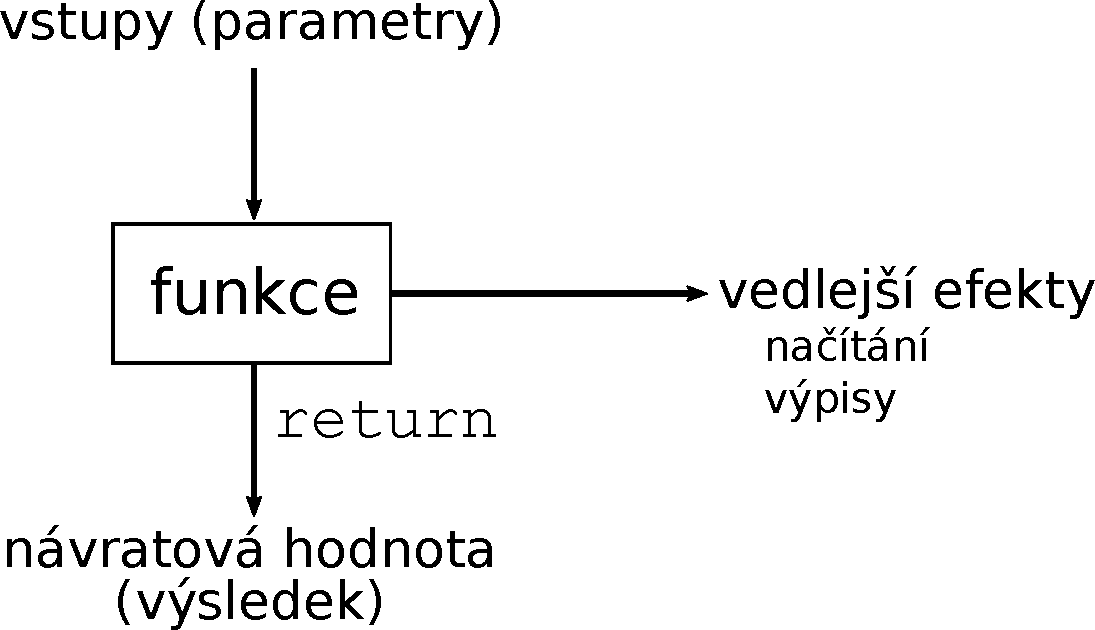
\includegraphics[width=8cm]{diagram.pdf}
\vspace{5mm}

Funkci v~konzolové aplikaci zapisujeme na stejnou úroveň, jako je funkce
\texttt{Main}:
\begin{verbatim}
static int MyFunc(int a, int b)
{
    if (a == 0)
        return 0;
    return a + b;
}
\end{verbatim}

Funkce v~konzolové aplikaci začíná slovem \texttt{static}, pak následuje typ
výsledku (v~našem případě \texttt{int}), pak následuje jméno funkce (mělo by
začínat velkým písmenem!) a pak jsou v~závorkách uvedeny parametry. Pak
následuje tělo funkce, ve kterém může být příkaz \texttt{return}.

Příkaz \texttt{return} způsobí ukončení funkce a vrácení hodnoty, která
je za příkazem.

Pokud jako typ návratové hodnoty zadáme \texttt{void}, funkce nic nevrací
(není třeba psát příkaz \texttt{return}).

Funkci můžeme zavolat:
\begin{verbatim}
MyFunc(5, 7);
\end{verbatim}

Můžeme si také uložit výsledek a vypsat jej:
\begin{verbatim}
int result = MyFunc(5, 7);
Console.WriteLine(result);
\end{verbatim}

Nebo zkráceně:
\begin{verbatim}
Console.WriteLine(MyFunc(5, 7));
\end{verbatim}

\end{document}
